\subsection{Word in Finite Field}

In order to make the processing logic of the VM simple, to obtain the smallest basic constraint unit (which can constrain any instruction of the VM), we defined the VM over a finite field so that the Word of the VM is a field element. Therefore, the calculation logic of the VM only supports a few simple field operations, such as addition, subtraction (equivalent to adding an additive inverse), multiplication, and division (equivalent to multiplying a multiplicative inverse). Meanwhile, we have also implemented integer calculation logic in order to support integer operations (OlaVM supports uint256 integer calculations to strengthen compatibility with Ethereum). The relationship between integer calculation and field calculation is shown in Figure \ref{fig:field-operation}.
\begin{figure}[!ht]
    \centering
    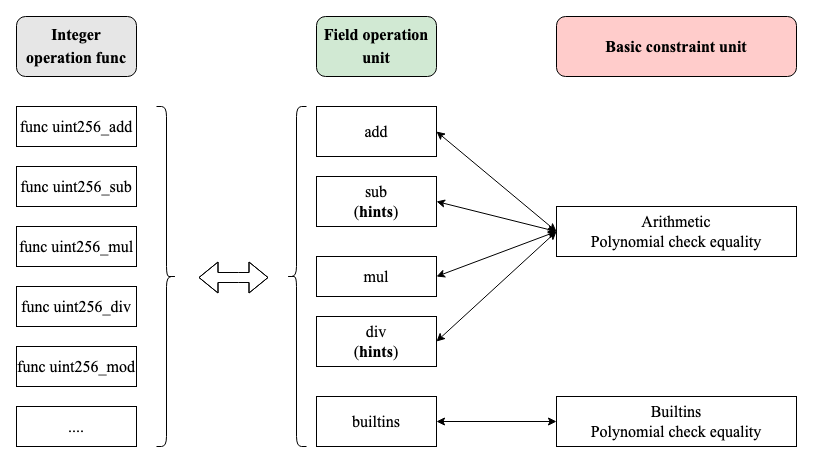
\includegraphics[width=0.6\textwidth]{field-operation.png}
    \caption{Field operation}
    \label{fig:field-operation}
\end{figure}

As you can tell, OlaVM instruction set defined over a finite field are very concise, with only a few instructions, hence the number of constraint units of the circuit will be very small. In PSE scheme, the underlying constraint unit needs to process the logic of all EVM instructions, which adds up to roughly 100 instructions, vastly increasing its complexity. In addition to this, we have defined some builtins in order to support more complex logic. Thanks to this, given complex calculations that needs to be implemented, we don't need to utilize these VM instructions, we can pre-implement the corresponding custom constraint logic and call that directly.

\emph{Note:} Current choice of finite field is BLS12-381 curve, which is planned to support uint256 integer calculations (refer to the design of StarkWare \cite{website:starkware}).
